\section{Experiments and Discussion}
\label{sec:exp}
\subsection{Debugging The Smooth Step}
%\textbf{Bug Description:}\\
%When the smooth step is added, the mixture of gaussian model won't expand to fit the input observations.\\
%\textbf{Test Case Generation:}\\
%In order to debug the problem, I generated a set of six synthetic point clouds. For the purpose of debugging, I deliberately made sure that the first 2657 points belonging to table, the following 2028 points belonging to chair, the last 3286 points belonging to teddy. The Test Cases are shown in Figure \ref{fig:syn-data}.
%\begin{figure}[ht]
%  \centering
%  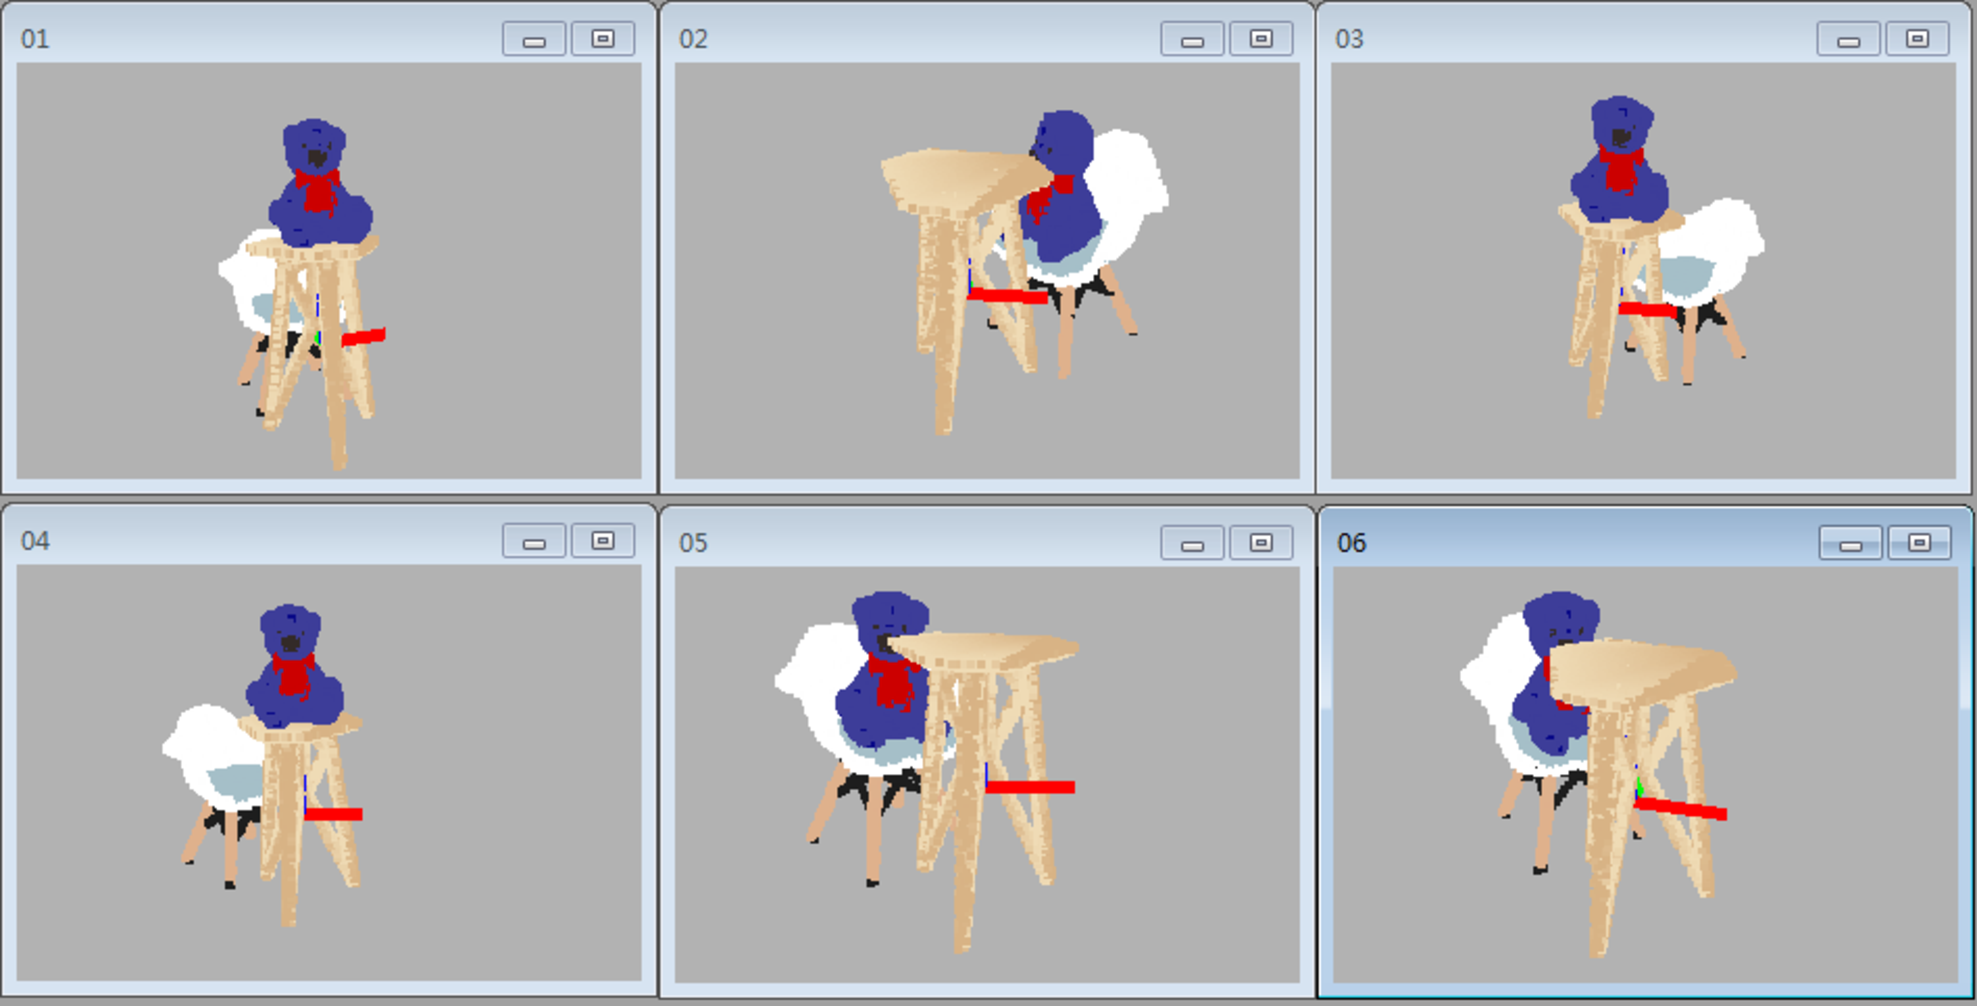
\includegraphics[width=3.0in]{images/synthetic_data}
%  \caption{The Synthetic Data for Test:they are composed of three objects (teddy table and chair) with different rigid motion}
%  \label{fig:syn-data}
%\end{figure}\\
%\textbf{The Example of $\alpha$:}\\
%The $\alpha$ are caculated as
%$$\alpha_{ijk}=p_np_kN(\phi_n(v_{ij})|x_k,\Sigma_k)$$
%The example $\alpha$ with no smooth:\\
%\begin{figure*}
%\centering
%	\subfigure[
%	$\alpha_0$,iteration 0
%	]{\label{fig:a0_0}
%		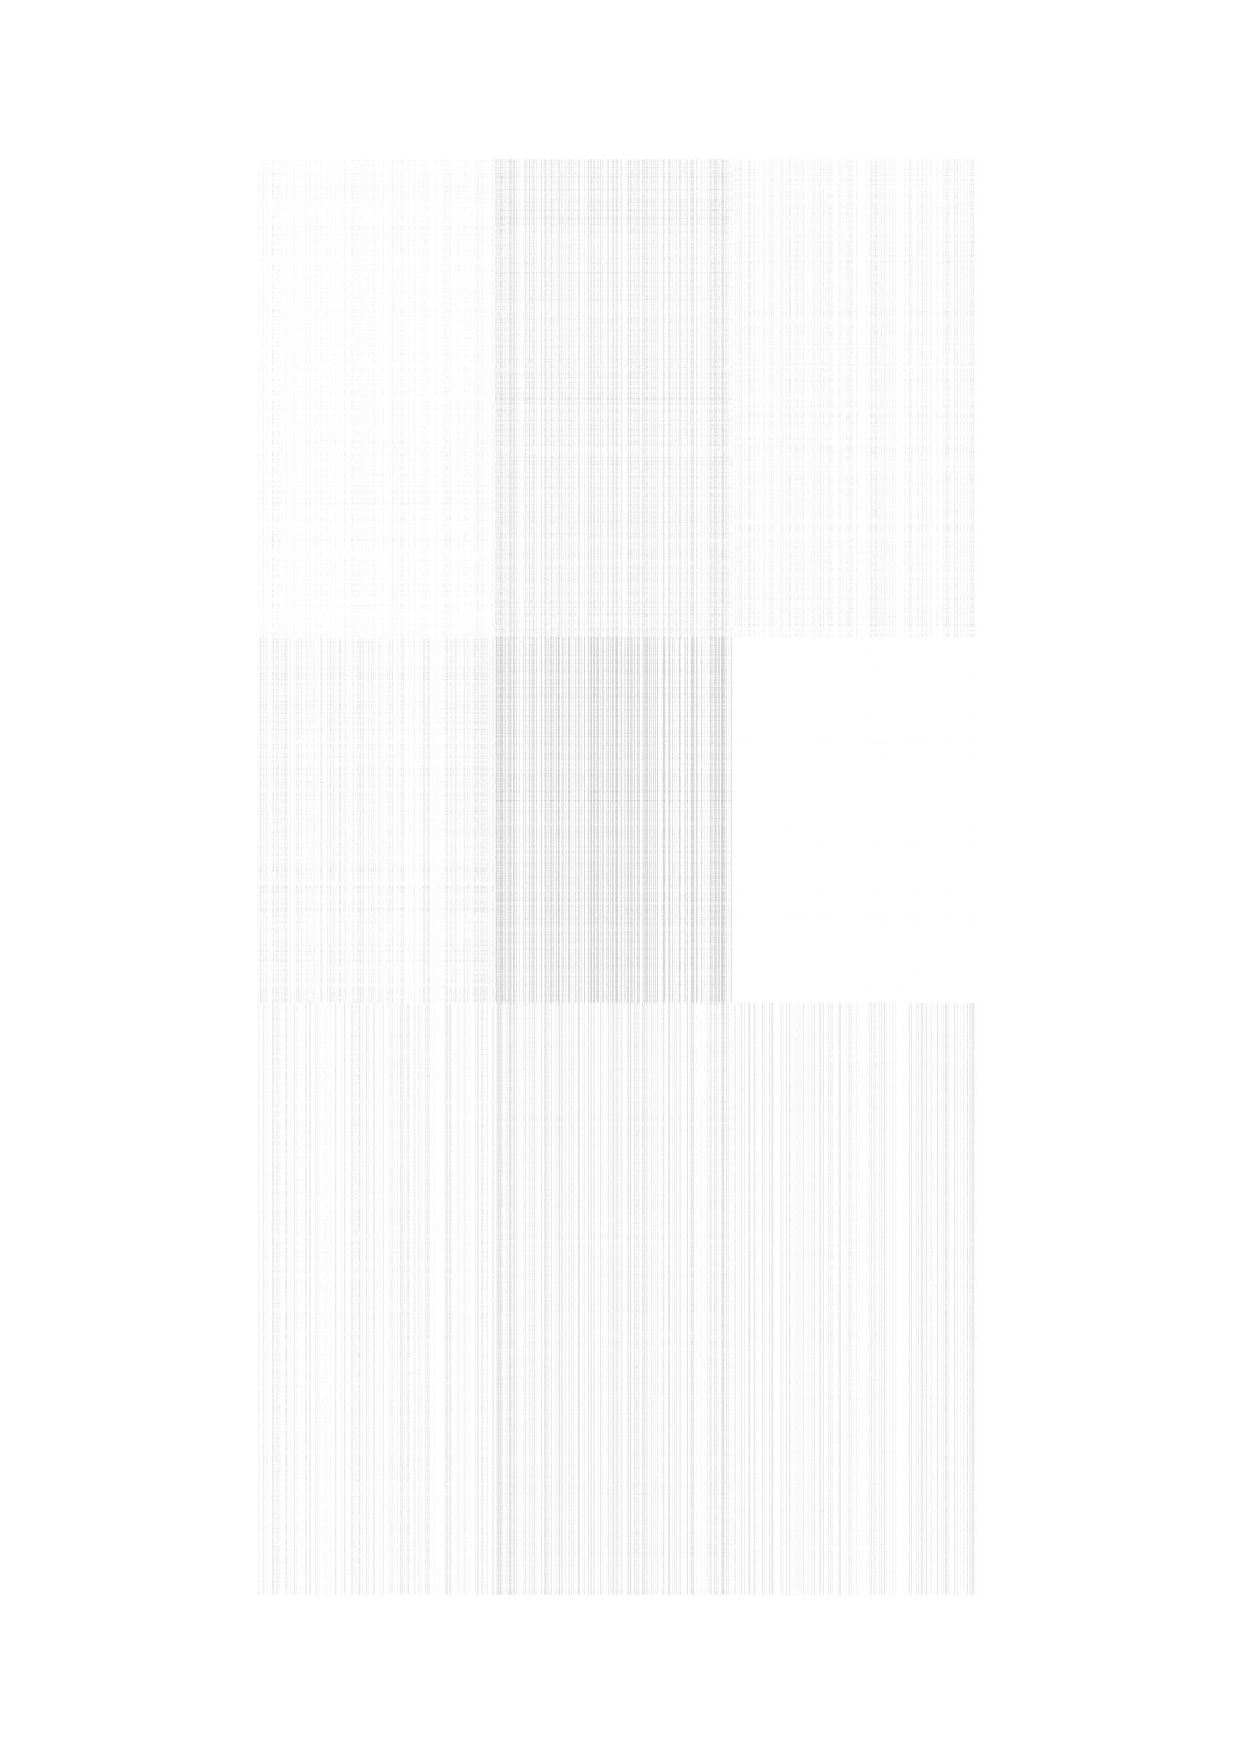
\includegraphics[width=0.3\textwidth]{images/alpha_0_iter_0.png}}
%	\subfigure[
%	$\alpha_0$,iteration 9
%	]{\label{fig:a0_9}
%		\includegraphics[width=0.3\textwidth]{images/alpha_0_iter_9.png}}
%	\subfigure[
%	$\alpha_0$,iteration 19
%		]{\label{fig:a0_19}
%		\includegraphics[width=0.3\textwidth]{images/alpha_0_iter_19.png}}
%	\subfigure[
%		$\alpha_1$,iteration 19
%		]{\label{fig:a1_19}
%		\includegraphics[width=0.18\textwidth]{images/alpha_1_iter_19.png}}
%	\subfigure[
%		$\alpha_2$,iteration 19
%		]{\label{fig:a2_19}
%		\includegraphics[width=0.18\textwidth]{images/alpha_2_iter_19.png}}
%	\subfigure[
%		$\alpha_3$,iteration 19
%		]{\label{fig:a3_19}
%		\includegraphics[width=0.18\textwidth]{images/alpha_3_iter_19.png}}
%	\subfigure[
%		$\alpha_4$,iteration 19
%		]{\label{fig:a4_19}
%		\includegraphics[width=0.18\textwidth]{images/alpha_4_iter_19.png}}
%	\subfigure[
%		$\alpha_5$,iteration 19
%		]{\label{fig:a5_19}
%		\includegraphics[width=0.18\textwidth]{images/alpha_5_iter_19.png}}
%	\caption{$\alpha$ with no smooth}
%	\label{fig:a_no_smooth}
%\end{figure*}
%as shown in Figure~\ref{fig:a_no_smooth}\\
%\textbf{The Problematic $\alpha$}
%\begin{figure*}
%	\centering
%	\subfigure[
%	$\alpha_0$,iteration 0
%	]{\label{fig:a0_0_smooth}
%		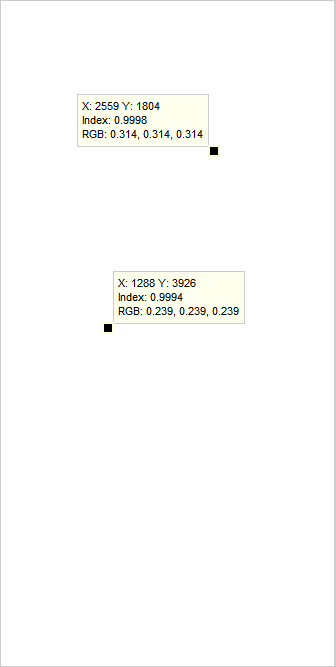
\includegraphics[width=0.3\textwidth]{images/alpha_0_iter_0_smooth.png}}
%	\subfigure[
%	$\alpha_1$,iteration 0
%	]{\label{fig:a1_0_smooth}
%		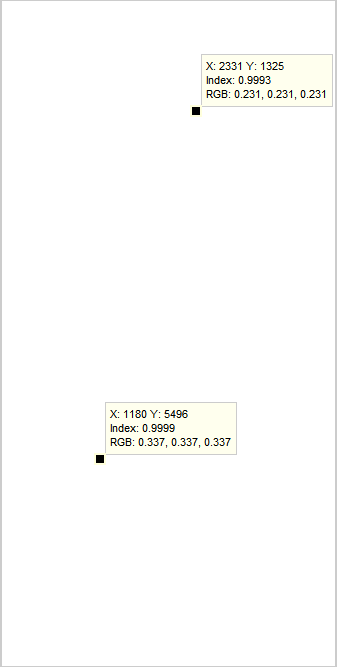
\includegraphics[width=0.3\textwidth]{images/alpha_1_iter_0_smooth.png}}
%	\caption{$\alpha$ after smooth}
%	\label{fig:a_smooth}
%\end{figure*}
\subsection{Current Result}
%As shown in Figure~\ref{fig:current_result}
%\begin{figure*}
%	\centering
%	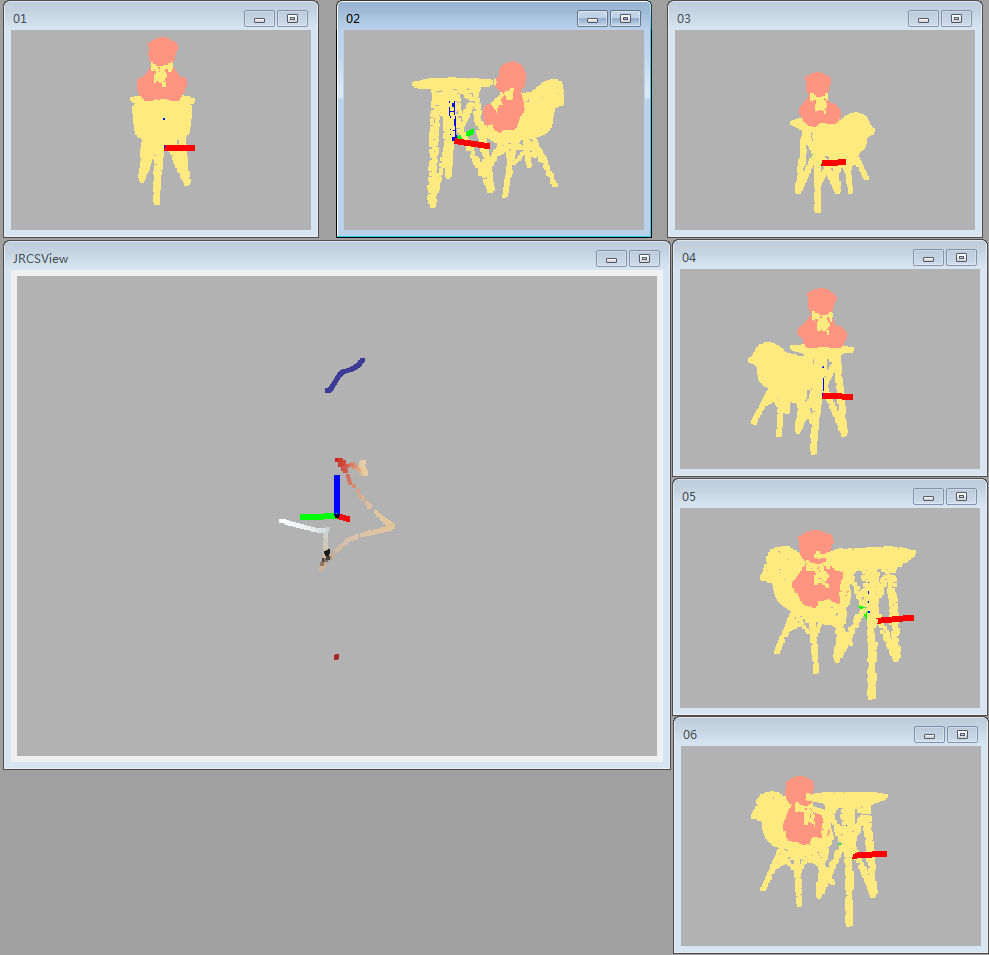
\includegraphics[width=\textwidth]{images/result_iter_18.png}
%	\caption{Current Result}
%	\label{fig:current_result}
%\end{figure*}\\
%\textbf{Current Alpha}\\
%\begin{figure*}
%	\centering
%	\subfigure[
%	$\alpha_0$,iteration 0
%	]{\label{fig:a0_0_0427}
%		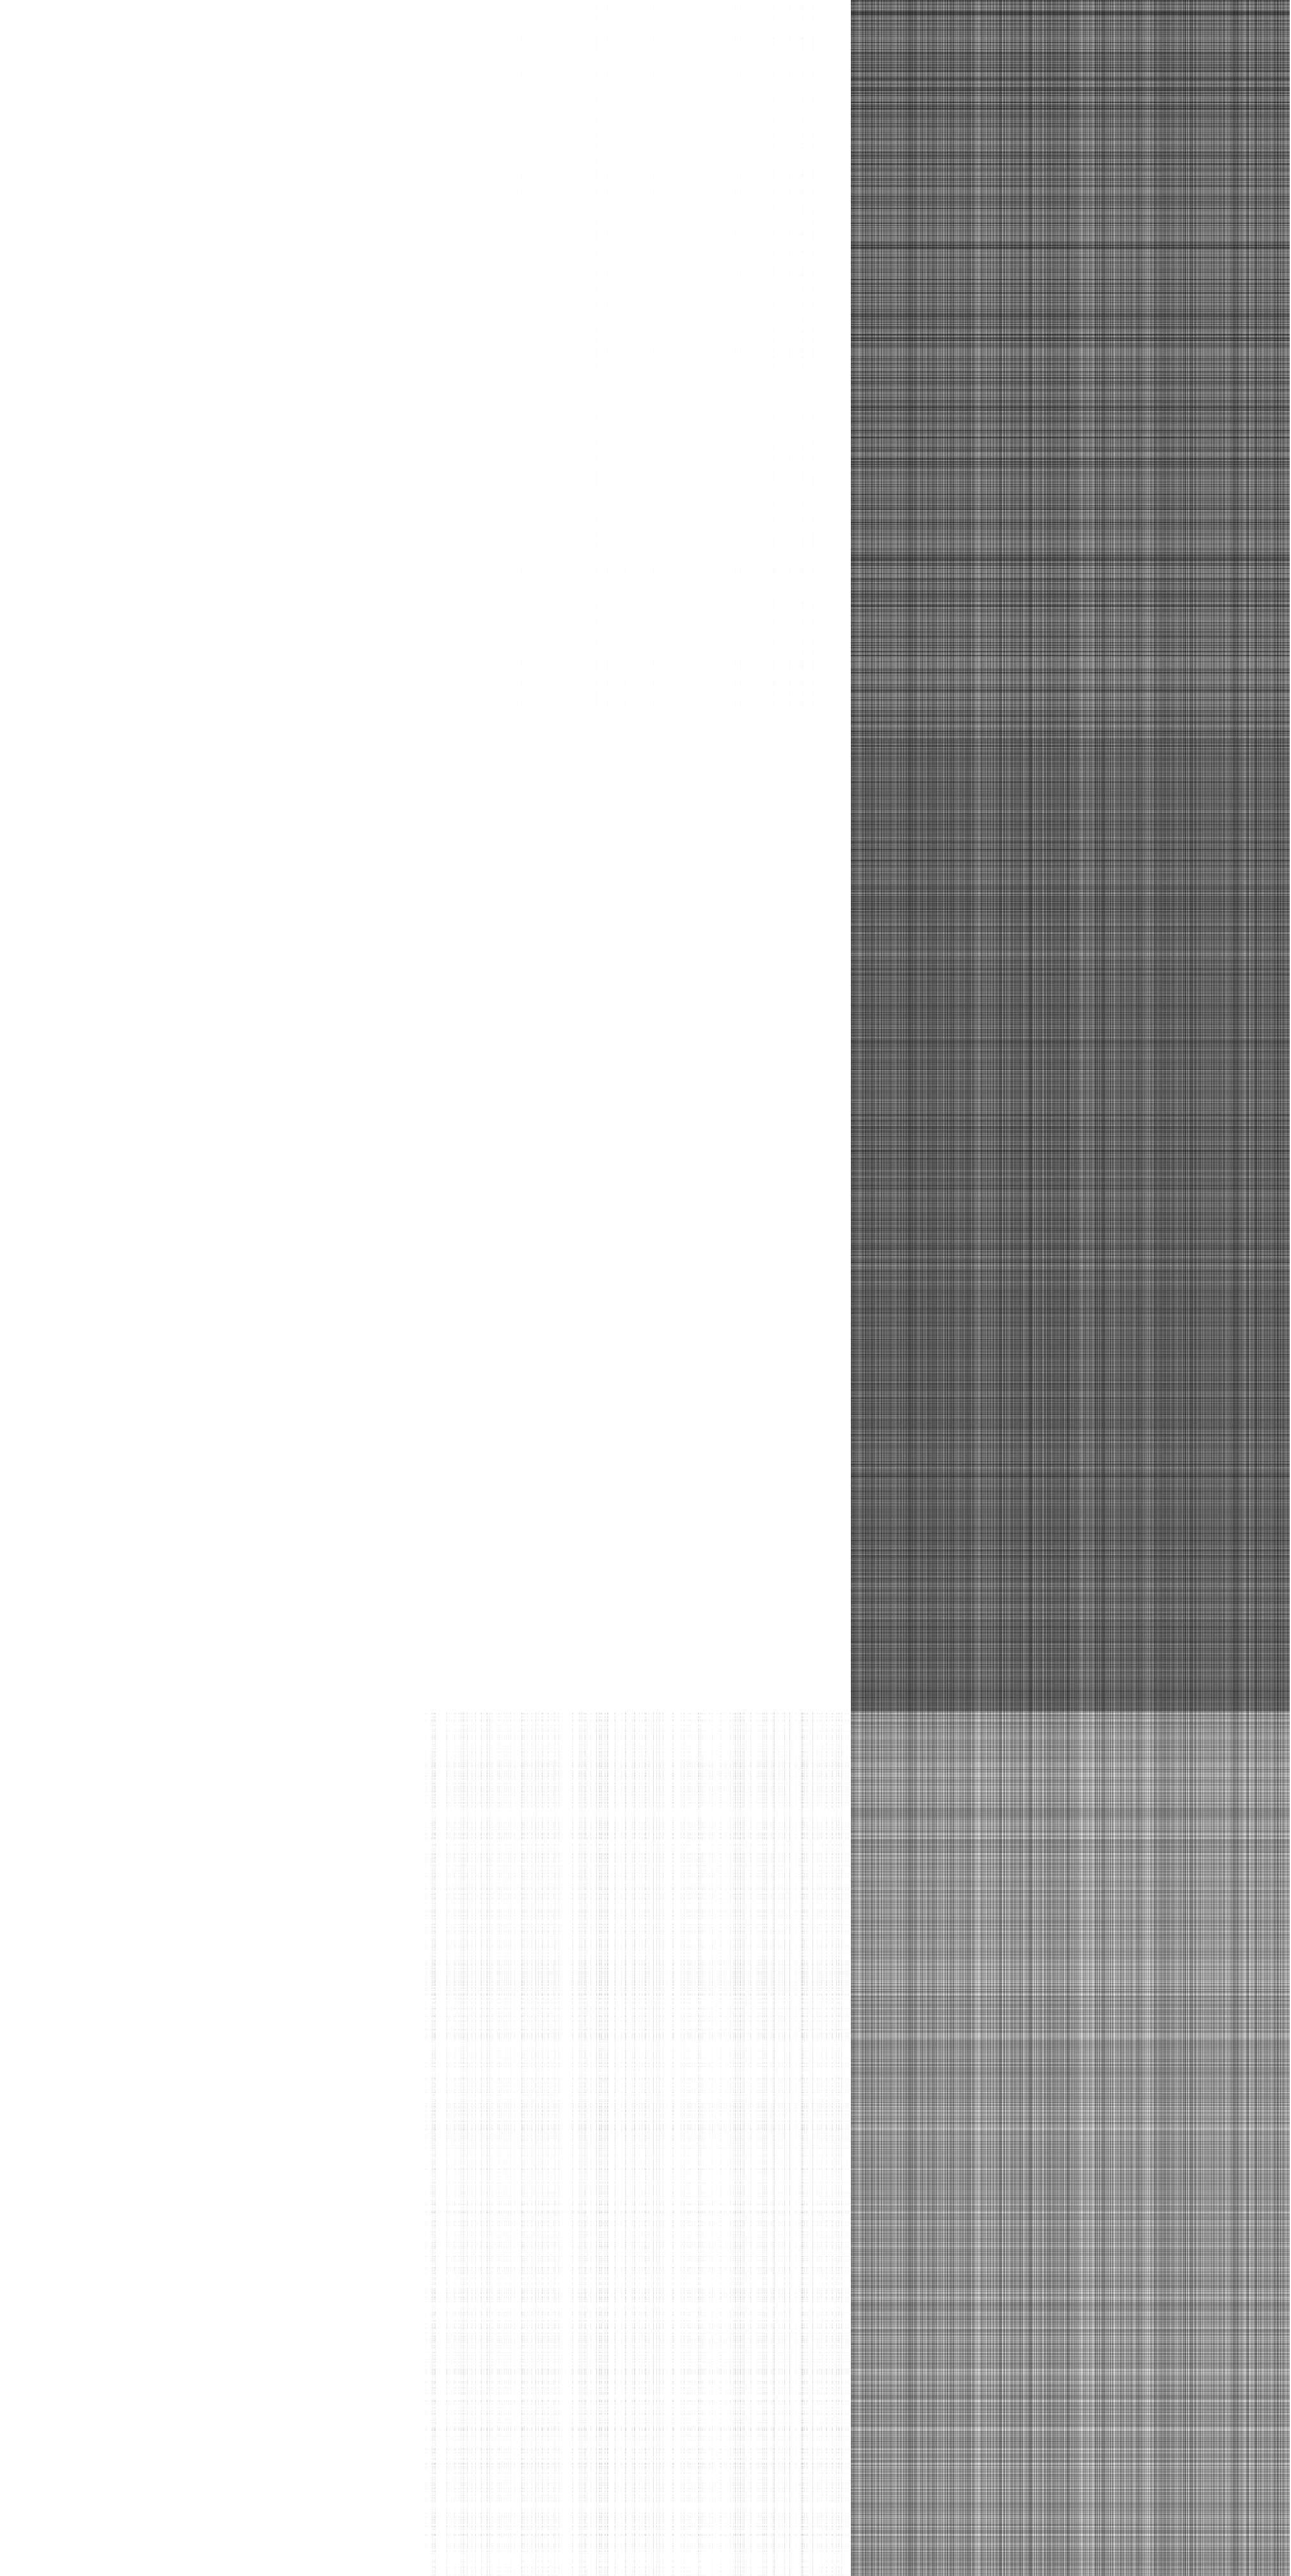
\includegraphics[width=0.3\textwidth]{images/alpha_0_iter_0_0427.png}}
%	\subfigure[
%	$\alpha_0$,iteration 9
%	]{\label{fig:a0_9_0427}
%		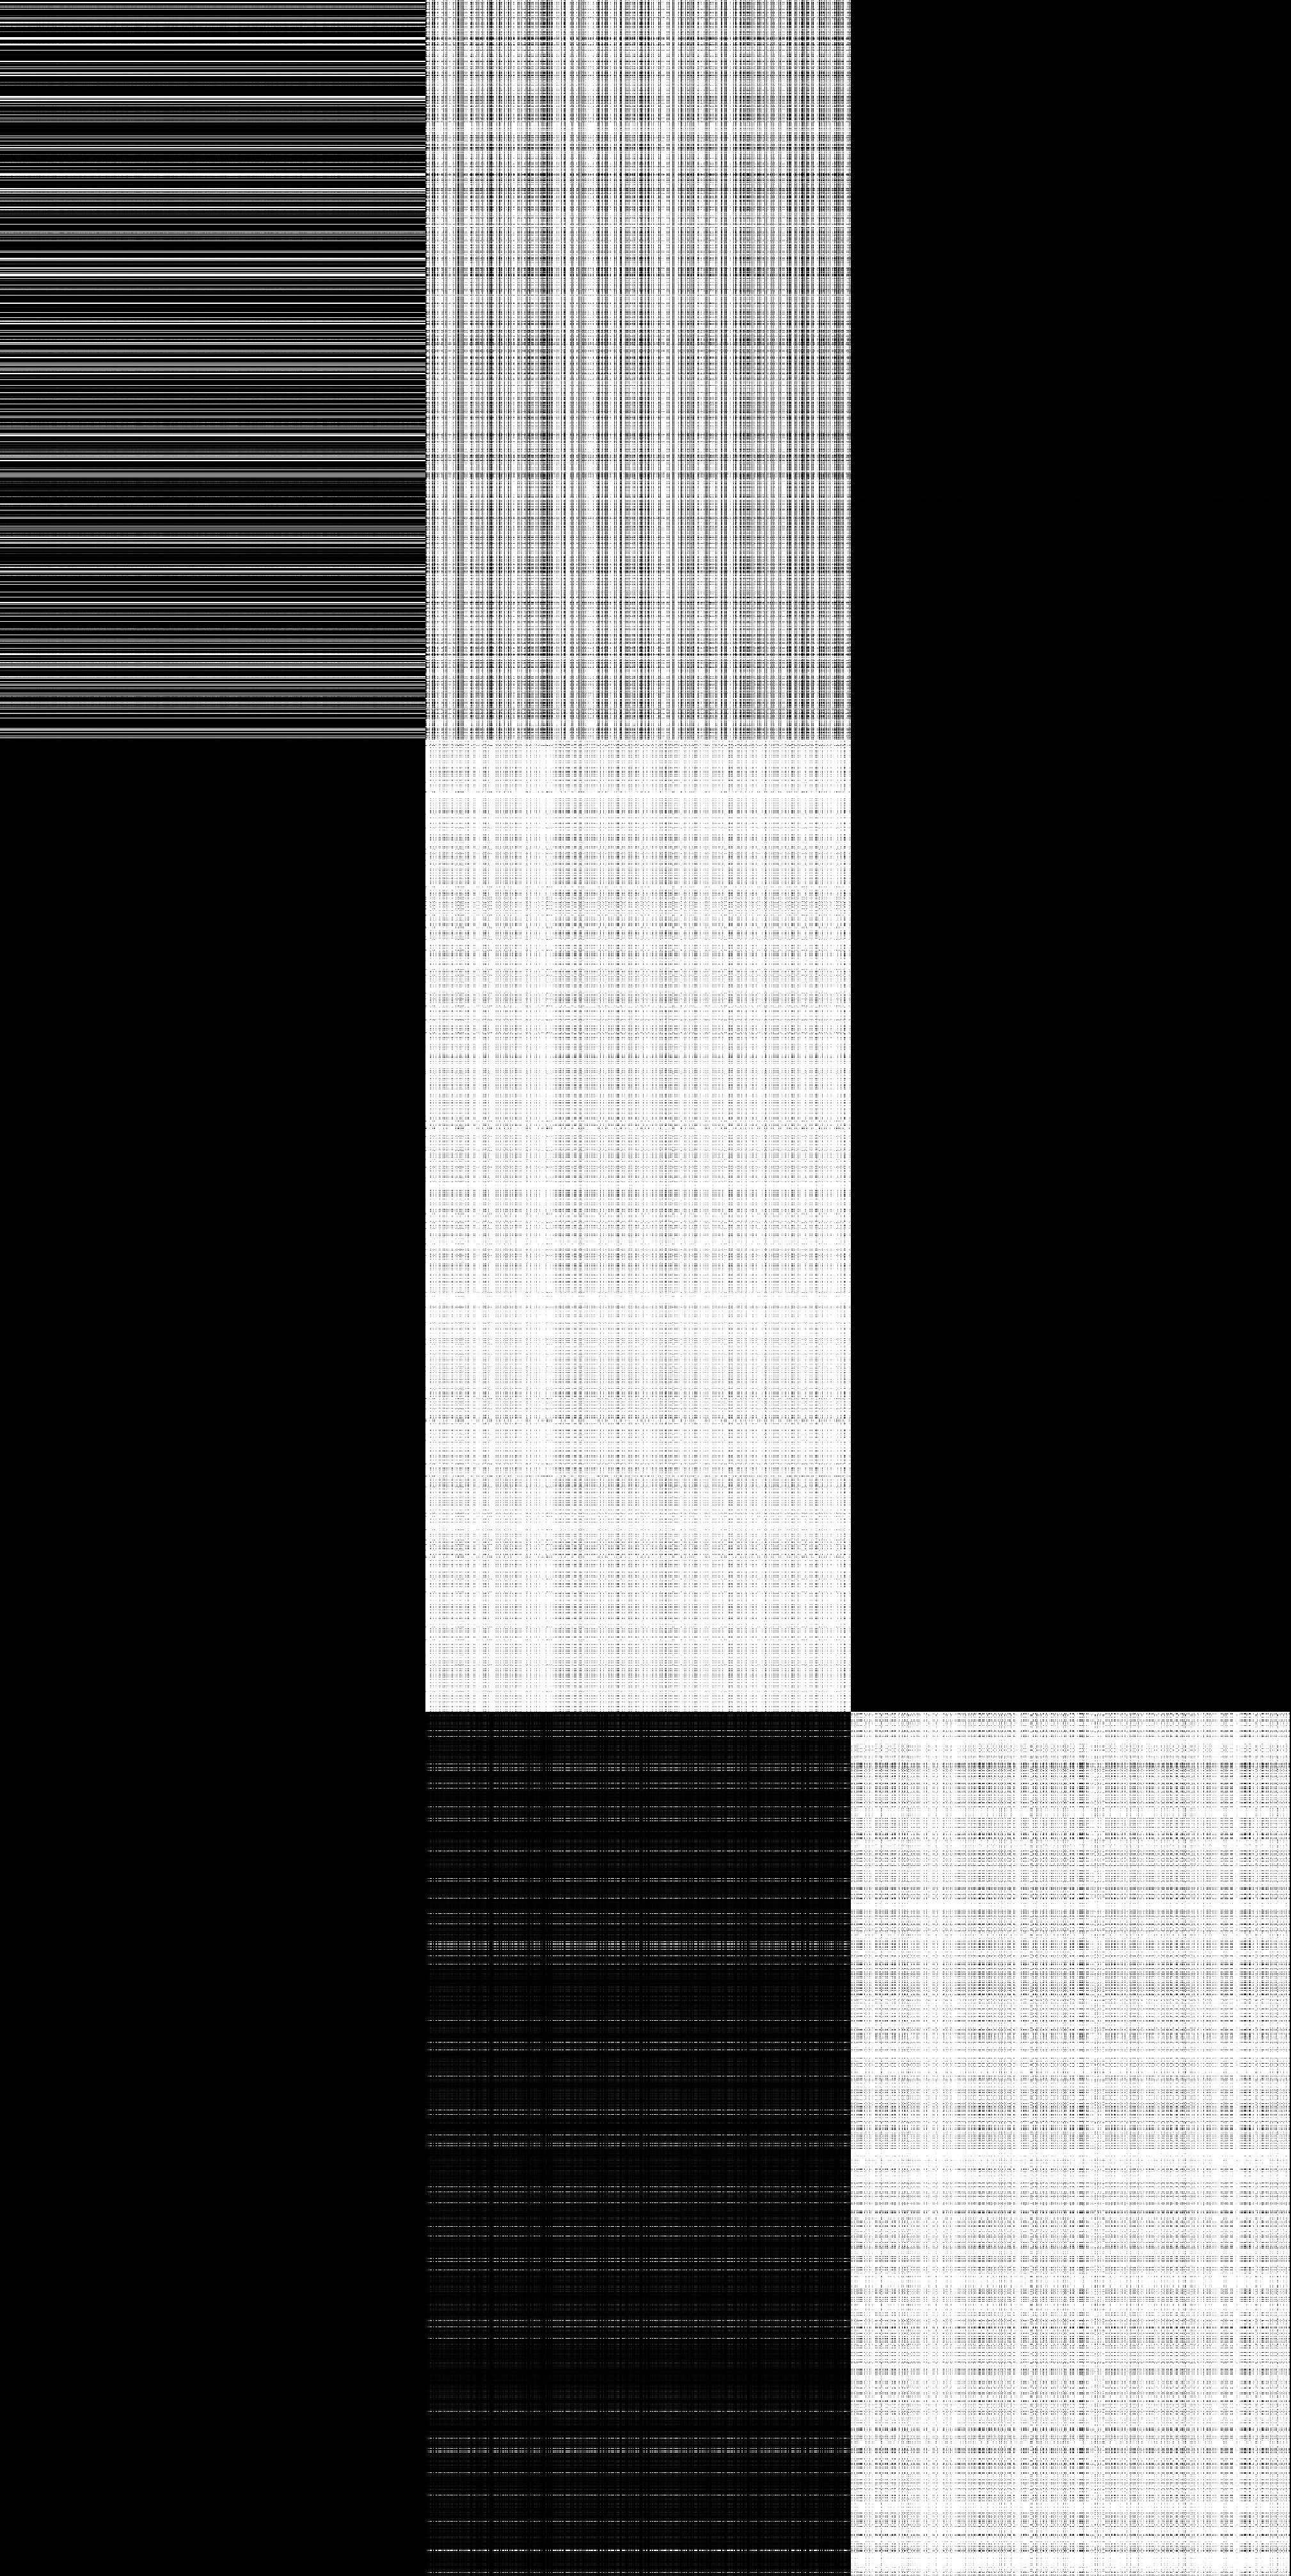
\includegraphics[width=0.3\textwidth]{images/alpha_0_iter_9_0427.png}}
%	\subfigure[
%	$\alpha_0$,iteration 19
%	]{\label{fig:a0_19_0427}
%		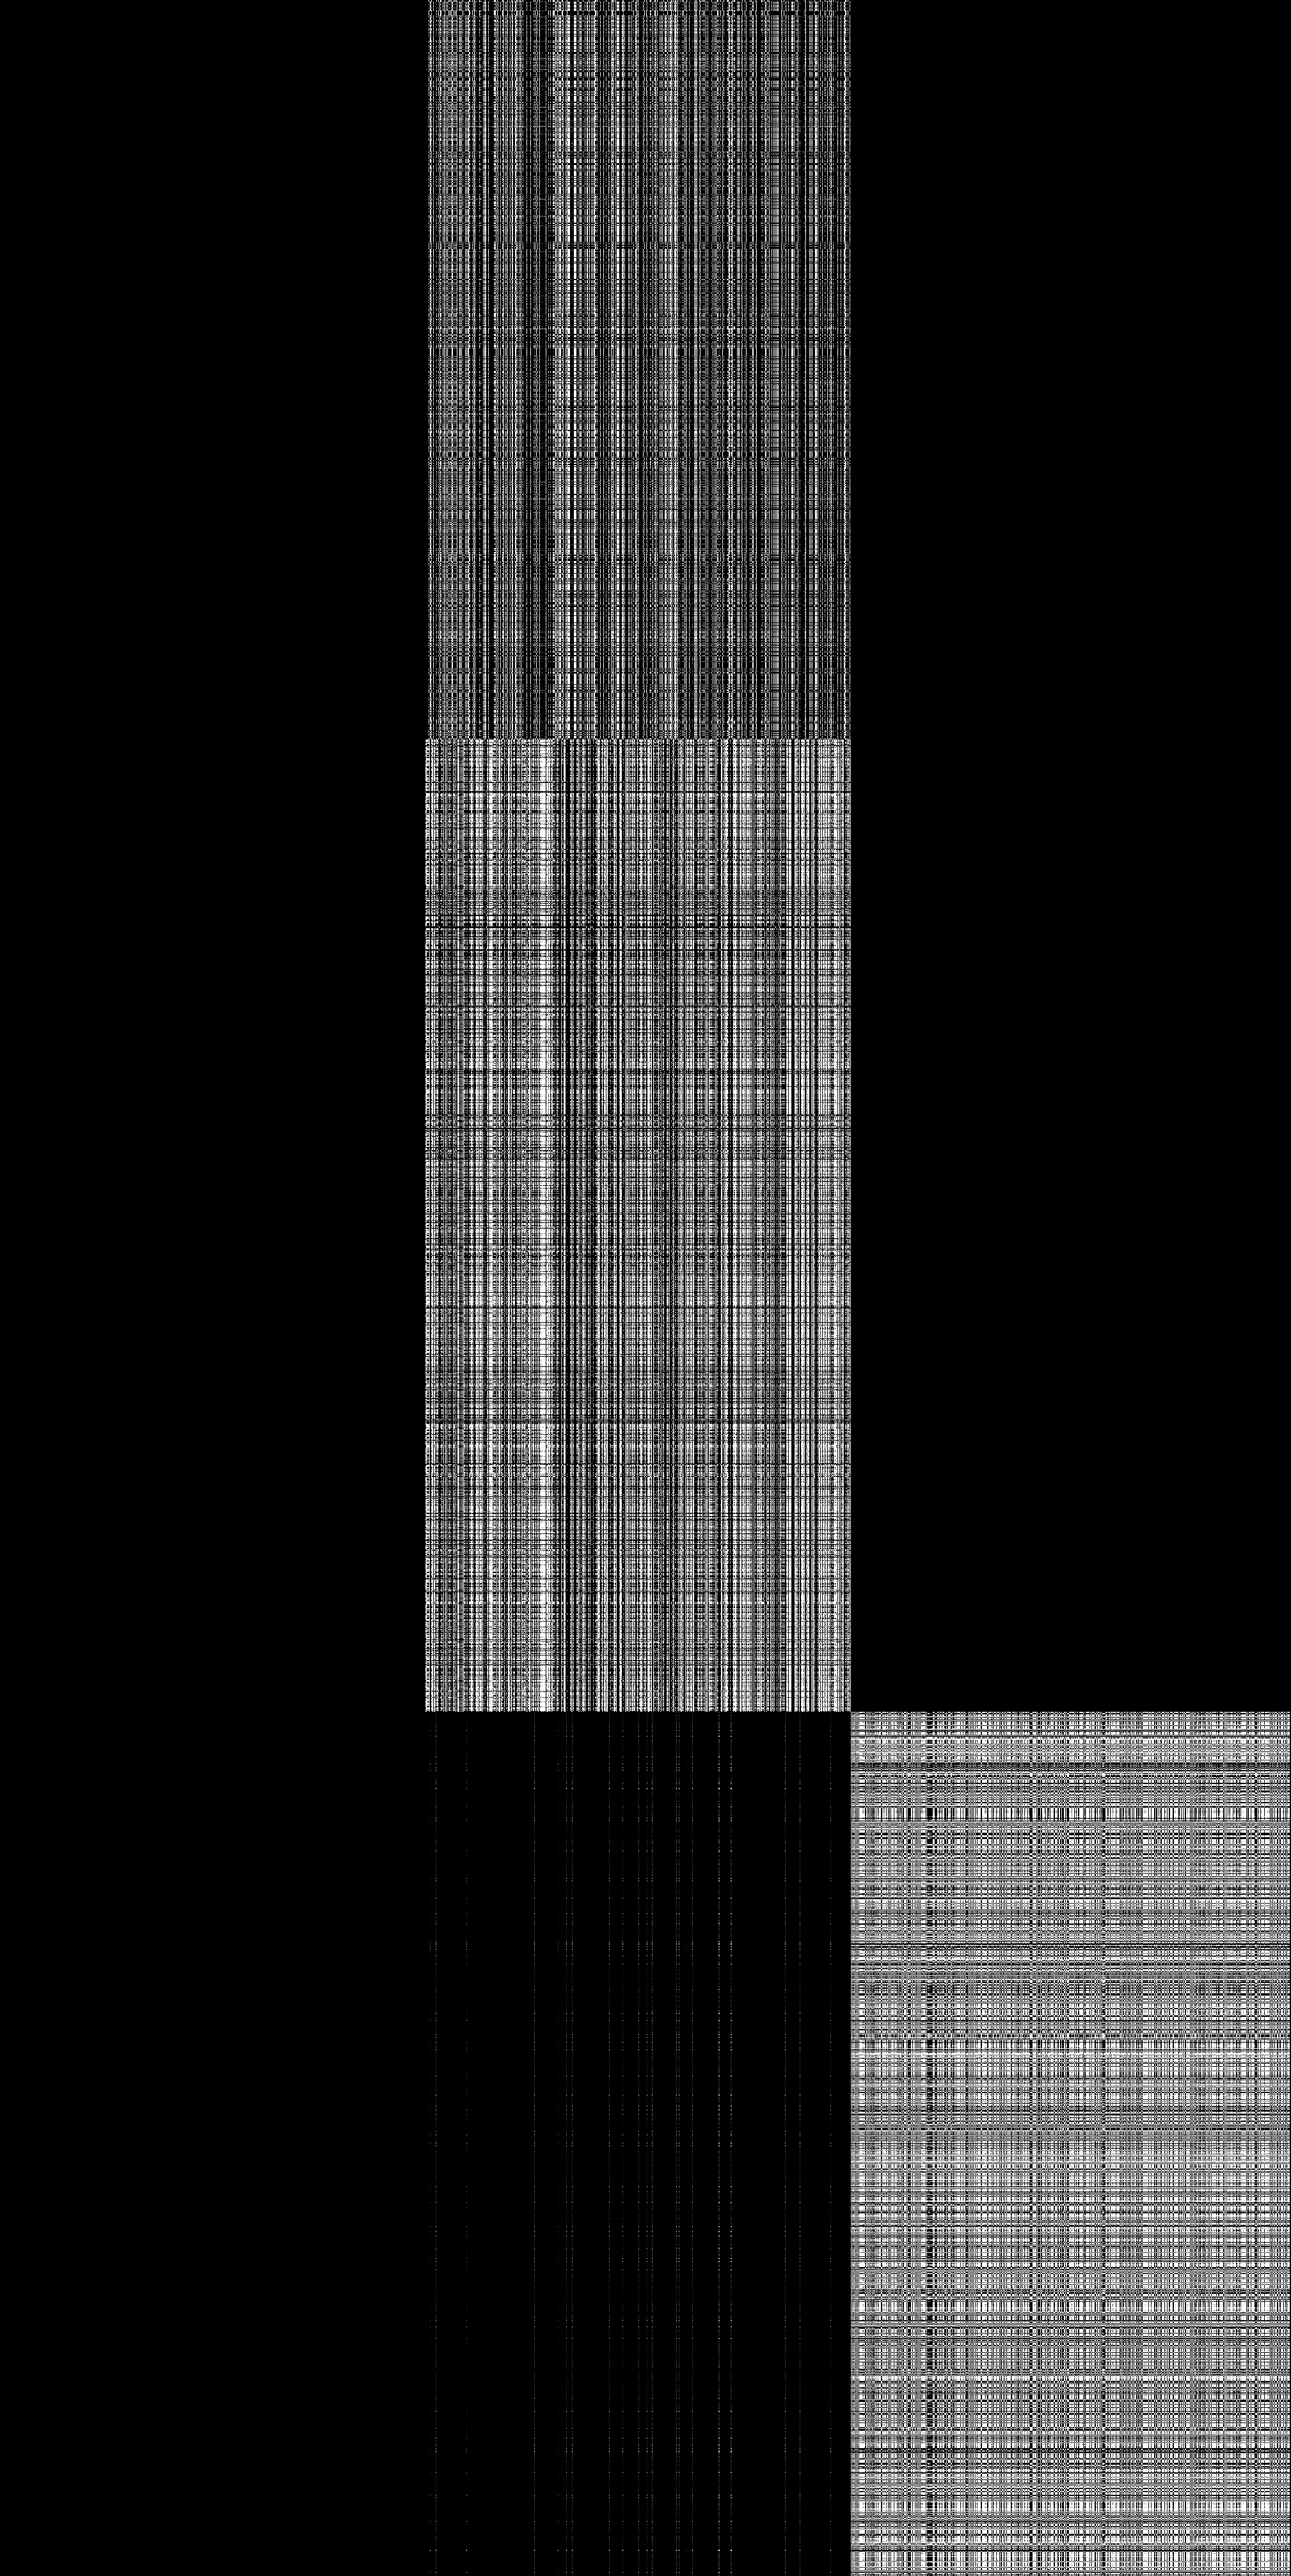
\includegraphics[width=0.3\textwidth]{images/alpha_0_iter_19_0427.png}}
%	\subfigure[
%	$\alpha_0$,iteration 0 smooth
%	]{\label{fig:a0_0_0427_smooth}
%		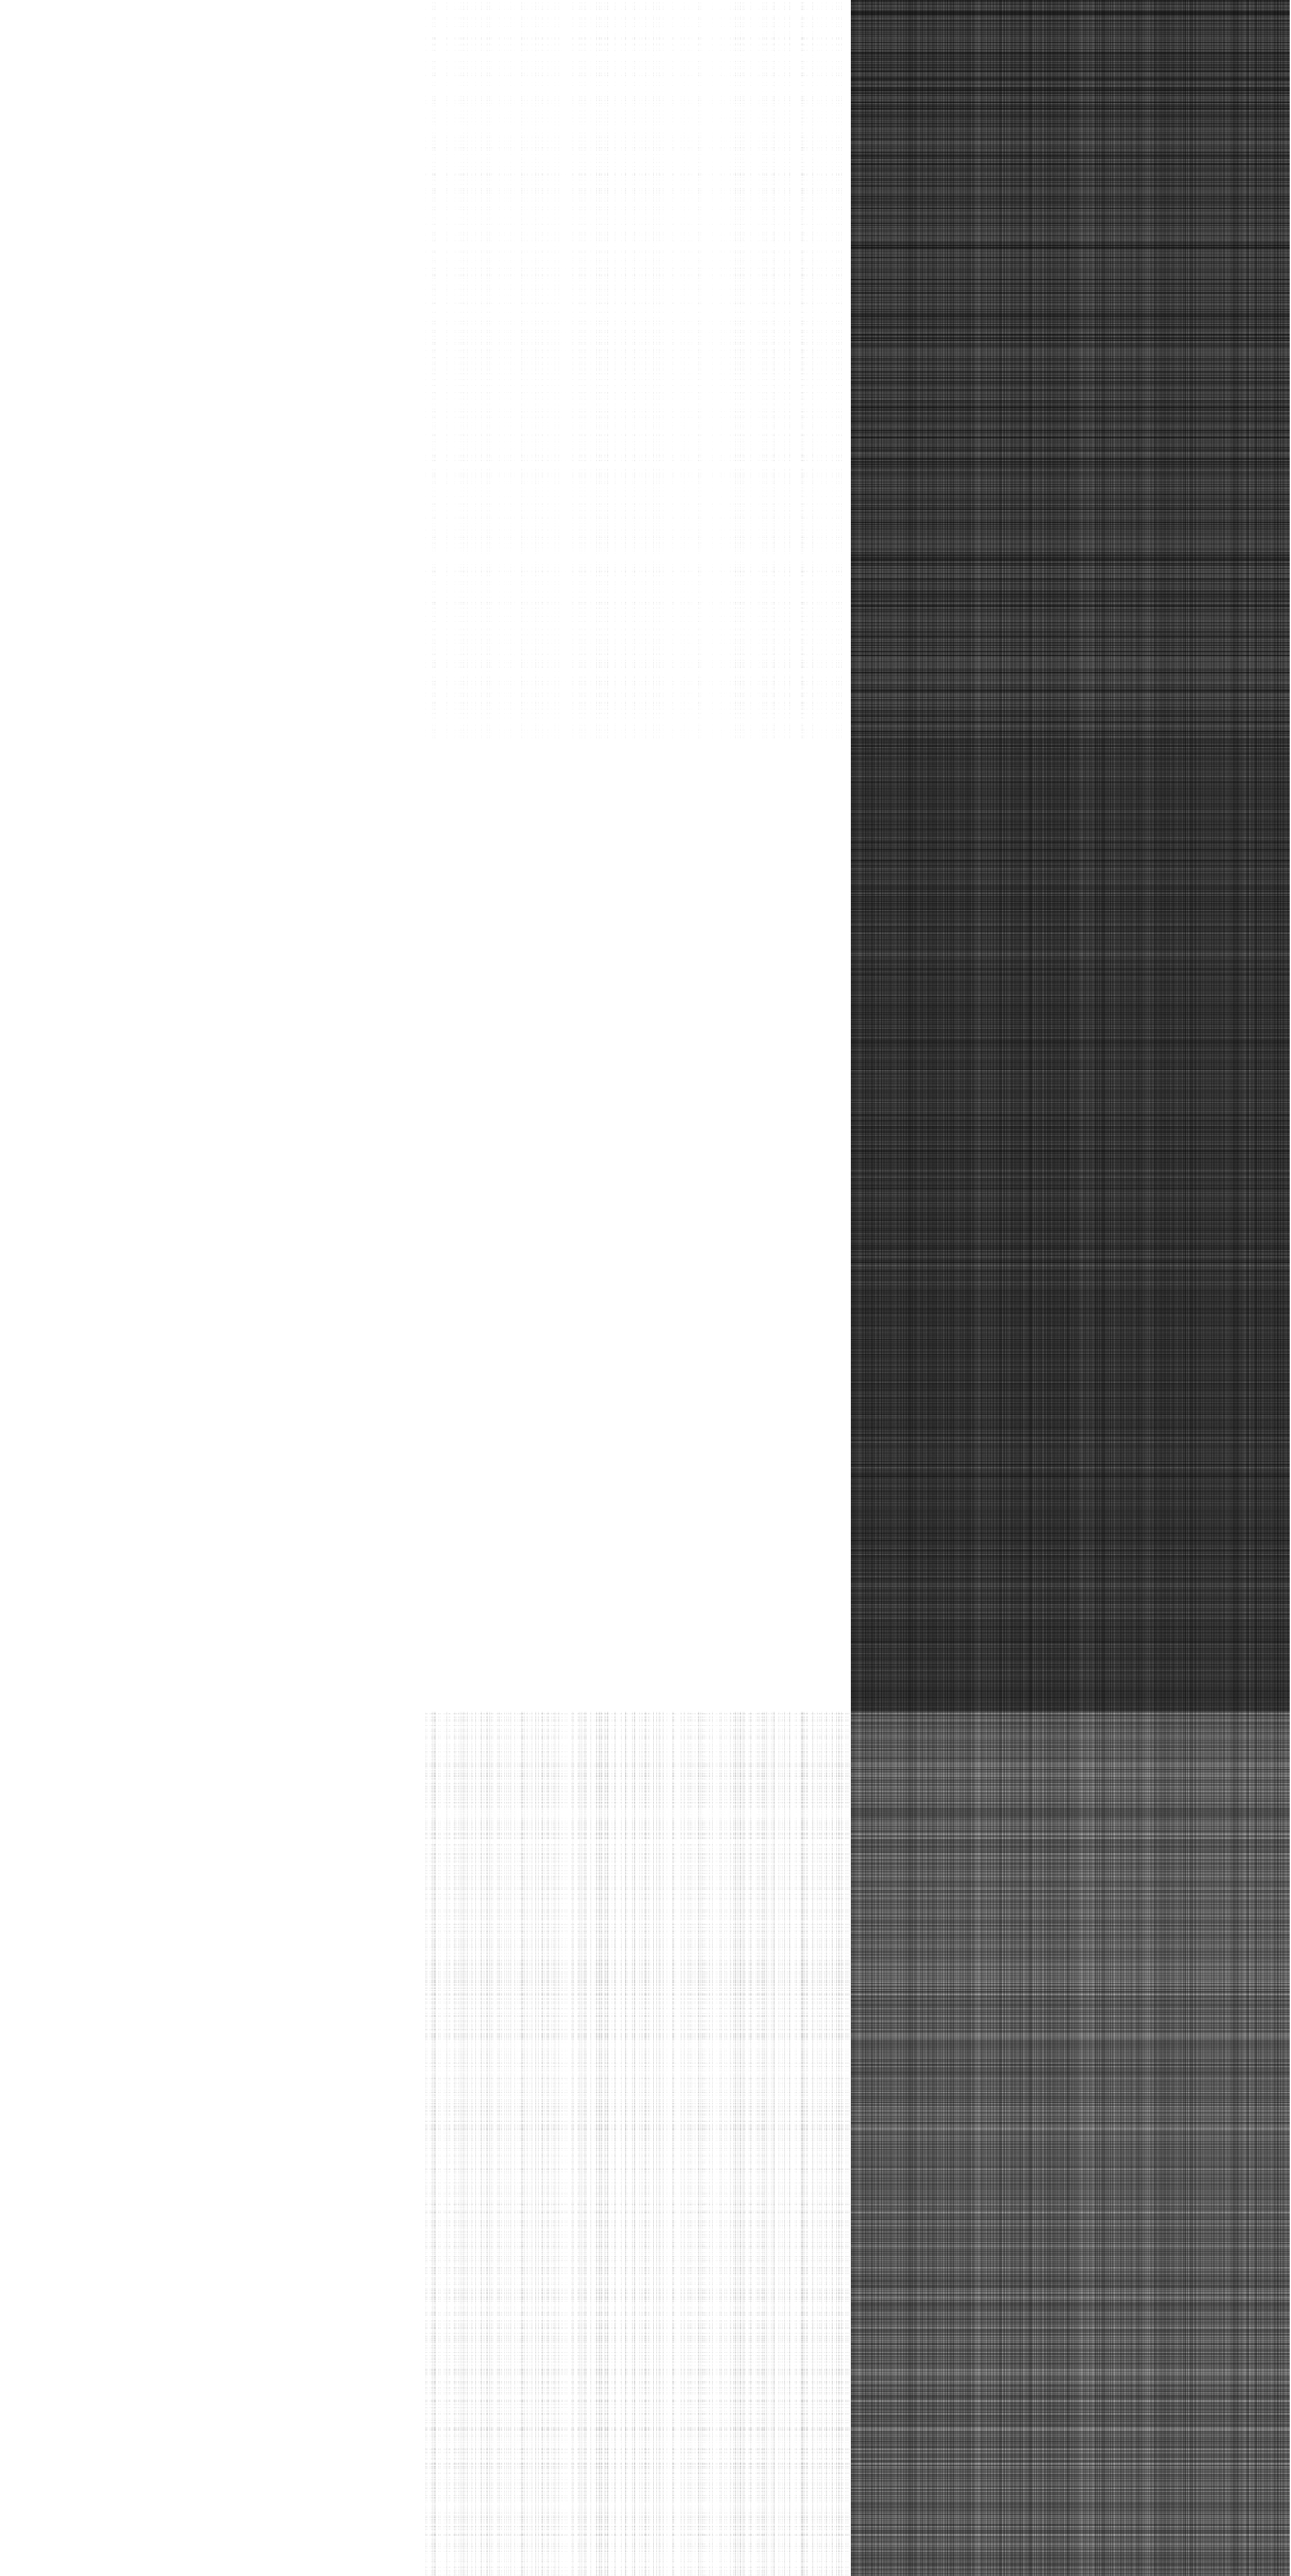
\includegraphics[width=0.3\textwidth]{images/alpha_0_iter_smooth_0_0427.png}}
%	\subfigure[
%	$\alpha_0$,iteration 9 smooth
%	]{\label{fig:a0_9_0427_smooth}
%		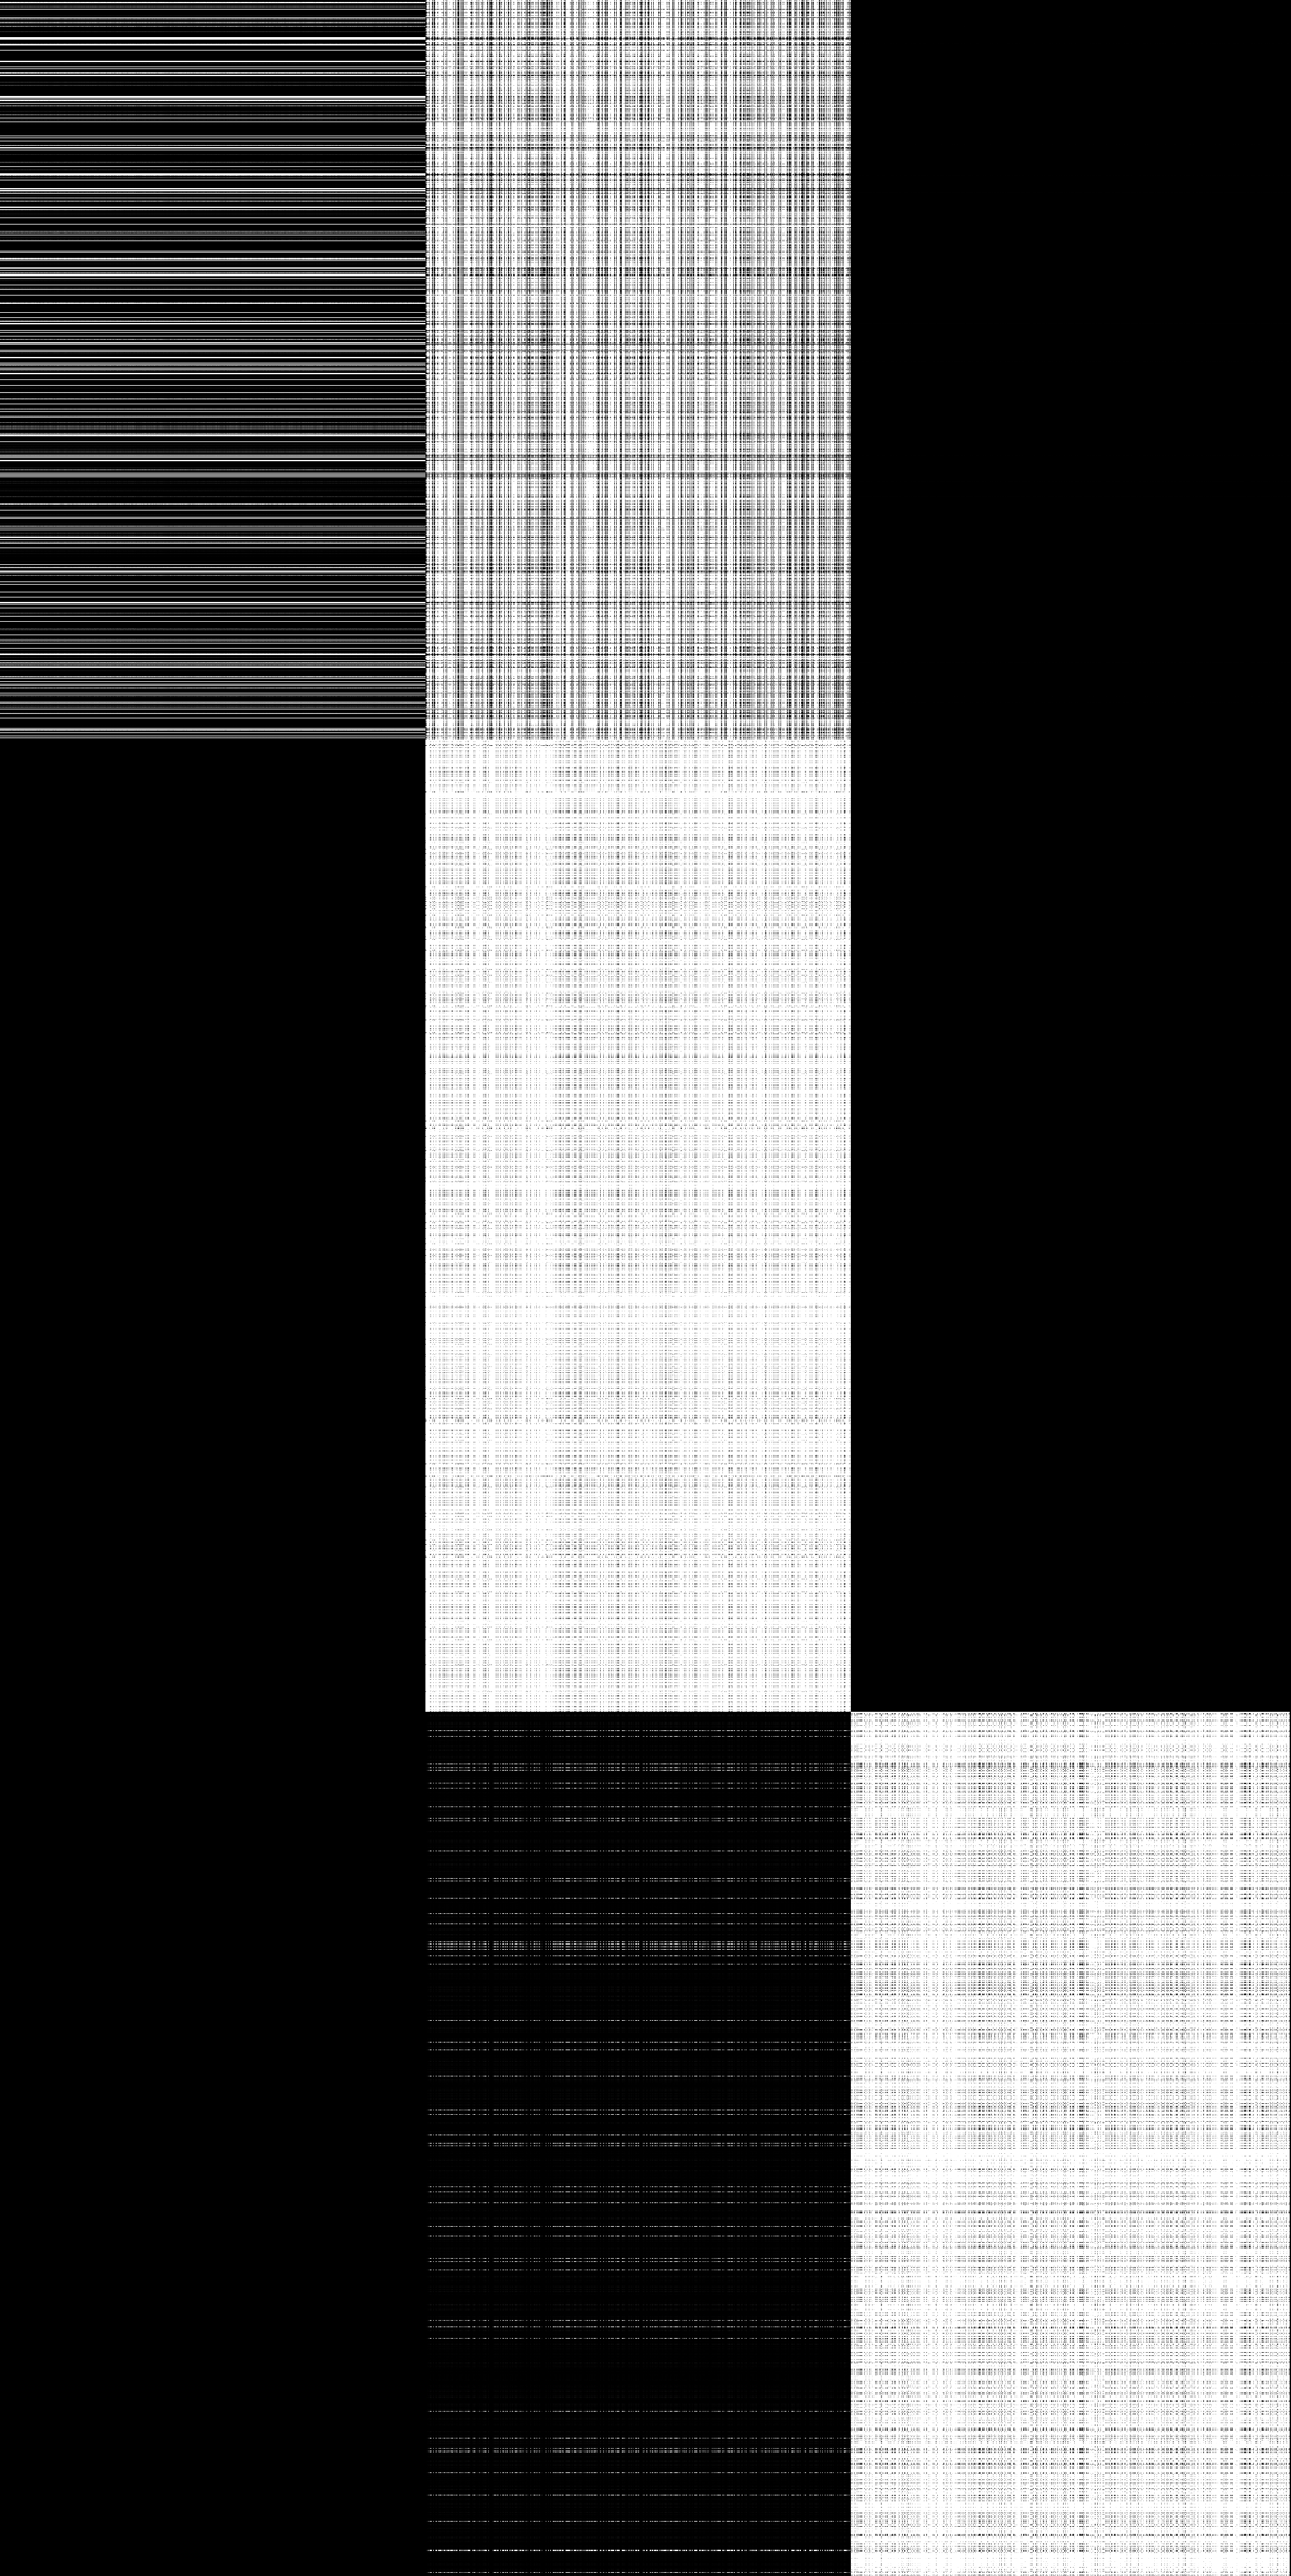
\includegraphics[width=0.3\textwidth]{images/alpha_0_iter_smooth_9_0427.png}}
%	\subfigure[
%	$\alpha_0$,iteration 19 smooth
%	]{\label{fig:a0_19_0427_smooth}
%		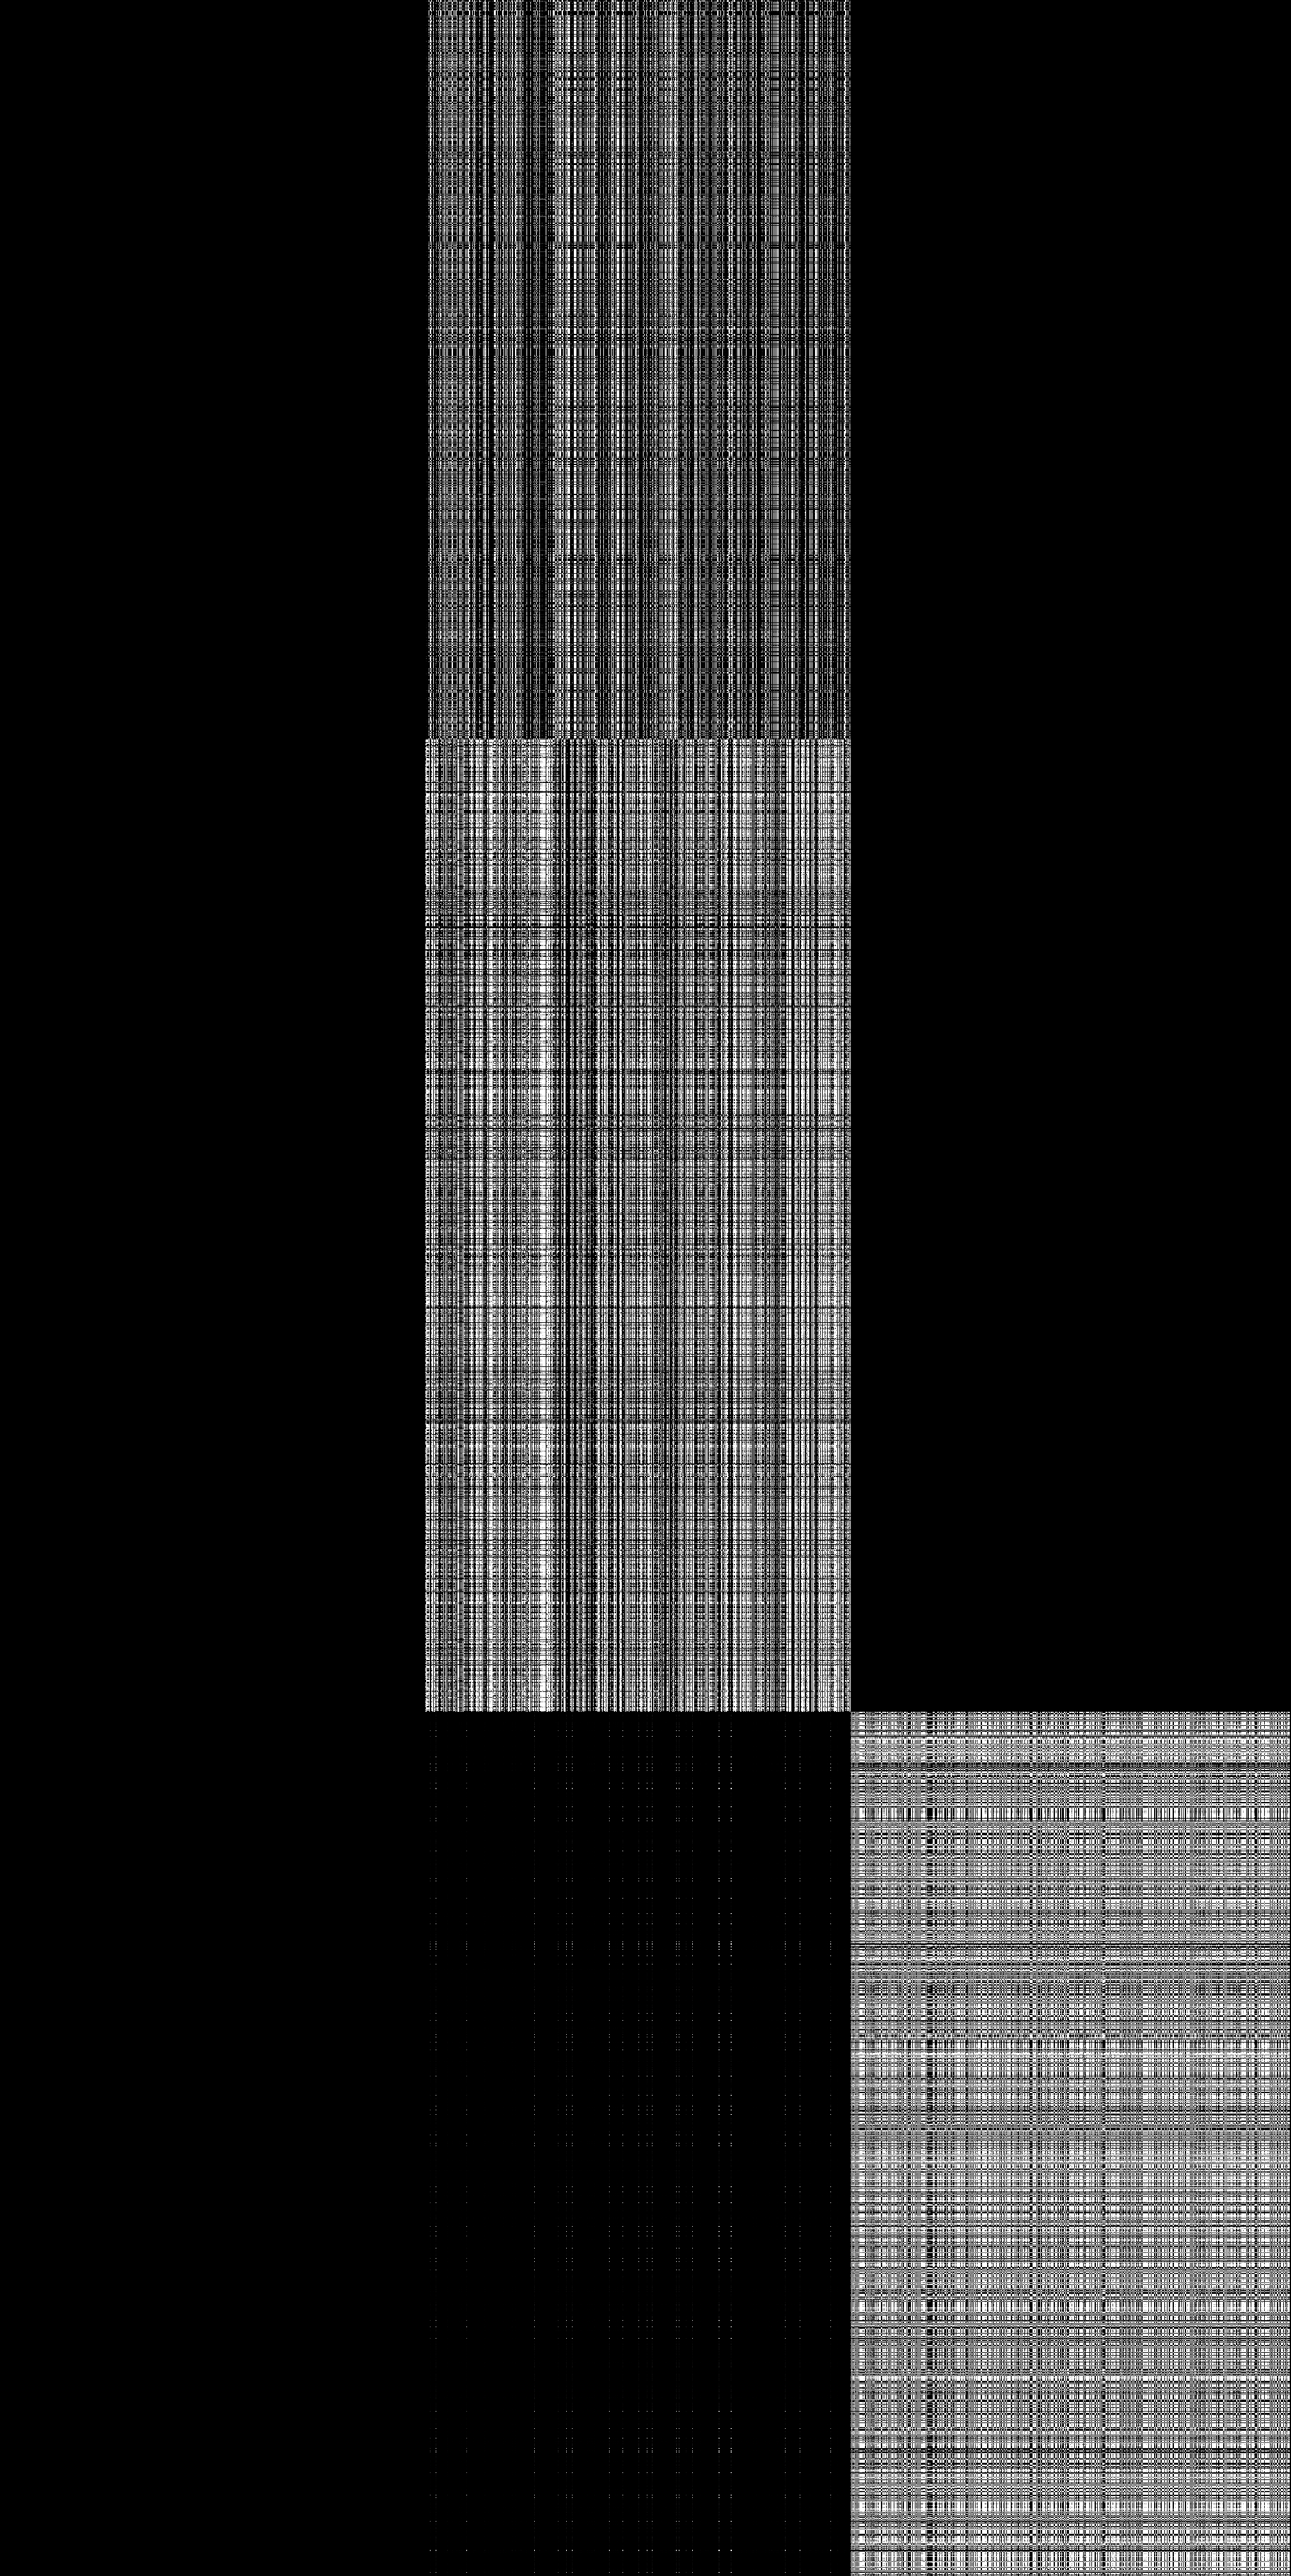
\includegraphics[width=0.3\textwidth]{images/alpha_0_iter_smooth_19_0427.png}}
%	\caption{$\alpha$ after smooth}
%	\label{fig:current_alpha}
%\end{figure*}
\subsection{Initialization Experiments}
\begin{figure*}
	\centering
	\includegraphics[width=\textwidth]{images/mannual_unified.png}
	\caption{Segments and mannully clustered result}
	\label{fig:input_for_init}
\end{figure*}
%\begin{figure*}
%	\centering
%	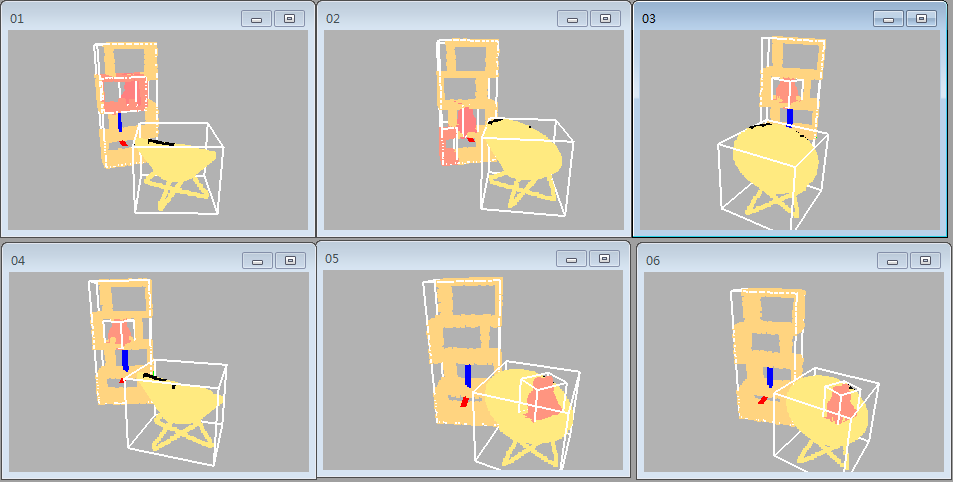
\includegraphics[width=\textwidth]{images/init_seg.png}
%	\caption{Segmentation for Initialization Experiments}
%	\label{fig:seg_for_init}
%\end{figure*}
%\begin{figure*}
%	\centering
%	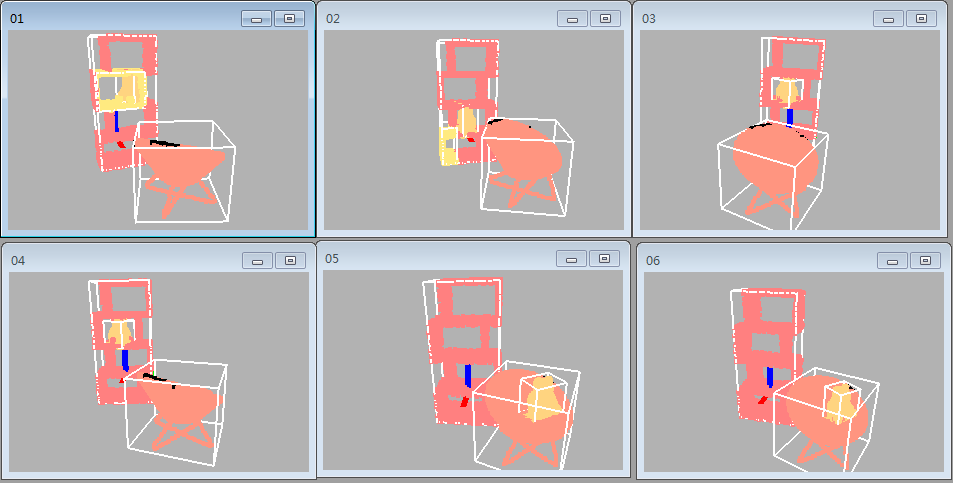
\includegraphics[width=\textwidth]{images/init_cluster.png}
%	\caption{Clustering for Initialization Experiments}
%	\label{fig:cluster_for_init}
%\end{figure*}
